\documentclass[a4paper]{article}

\usepackage[UTF8]{ctex}
\usepackage[a4paper,margin=1in]{geometry}
\usepackage{graphicx}
\usepackage{float}
\usepackage{listings}
\usepackage{longtable}
\usepackage{booktabs}
\usepackage{hyperref}
\usepackage{fancyhdr}
\usepackage{lastpage}
\usepackage{color}
\usepackage{indentfirst}        % 首段缩进
\setlength{\parindent}{2em}     % 缩进2字符
\usepackage{zhnumber}           % 中文编号
\usepackage[dvipsnames]{xcolor}
\usepackage{amsmath}
\newcommand{\college}{中山大学计算机学院}
\newcommand{\projname}{机器学习与数据挖掘|作业五}
\newcommand{\reporttitle}{Principal Component Analysis}
\newcommand{\stuno}{23336179}
\newcommand{\authorname}{马福泉}
\newcommand{\major}{计算机科学与技术}
\newcommand{\adviser}{梁上松}
\newcommand{\startdate}{2025年11月11日}
\newcommand{\labenddate}{2025年11月12日}
\newcommand{\labroom}{c206}

\pagestyle{fancy} % 使用 fancyhdr 风格
\fancyhf{}      % 清空默认的页眉页脚

% 设置页眉
\fancyhead[L]{\kaishu \projname}      % 左侧页眉显示项目名称
\fancyhead[C]{\kaishu \reporttitle}    % 中间页眉显示报告标题
\fancyhead[R]{\kaishu \authorname} % 右侧页眉显示作者姓名

% 设置页脚
\fancyfoot[C]{第 \thepage 页，共 \pageref{LastPage} 页} % 中间页脚显示页码

% 去除页眉页脚与正文之间的分隔线
\renewcommand{\headrulewidth}{0.4pt}
\renewcommand{\footrulewidth}{0pt}

% 设置文档背景颜色
\definecolor{mybgcolor}{RGB}{0, 0, 0} % 定义背景颜色
\definecolor{NavyBlue}{RGB}{0,0,128} % 添加颜色定义
% \pagecolor{mybgcolor} % 设置背景颜色

% listing 配置
\lstset{
    language=Python,
    basicstyle=\ttfamily\small,
    keywordstyle=\color{blue},
    commentstyle=\color{gray},
    stringstyle=\color{red},
    numbers=left,
    numberstyle=\tiny\color{gray},
    stepnumber=1,
    numbersep=5pt,
    backgroundcolor=\color{white},
    showspaces=false,
    showstringspaces=false,
    showtabs=false,
    frame=single,
    rulecolor=\color{black},
    tabsize=2,
    captionpos=b,
    breaklines=true,
    breakatwhitespace=false,
    escapeinside={\%*}{*)},
    extendedchars=false,
    inputencoding=utf8
}

\begin{document}

% 封面
\begin{titlepage}
    \centering
    

    
\includegraphics[width=10cm]{img/SYSULogo.png}

    \vspace{1em}
    %{\Large \college \par}
    \vspace{1em}
    {\Large \kaishu \projname \par}
    \vspace{3em}

    

    
    {\fontsize{40pt}{42pt}\kaishu \selectfont \boldmath \reporttitle\par}
    \vspace*{\fill}

    \begin{center}
    {\Large
    \makebox[5em][s]{学号}:\underline{\makebox[15em][c]{\kaishu \stuno}}\\[1em]
    \makebox[5em][s]{姓名}:\underline{\makebox[15em][c]{\kaishu \authorname}}\\[1em]
    \makebox[5em][s]{专业}:\underline{\makebox[15em][c]{\kaishu \major}}\\[1em]
    \makebox[5em][s]{课程教师}:\underline{\makebox[15em][c]{\kaishu \adviser}}\\[1em]
    \makebox[5em][s]{起始日期}:\underline{\makebox[15em][c]{\kaishu \startdate}}\\[1em]
    \makebox[5em][s]{结束日期}:\underline{\makebox[15em][c]{\kaishu \labenddate}}\\[1em]
    \makebox[5em][s]{实验地点}:\underline{\makebox[15em][c]{\kaishu \labroom}}
    }
    \end{center}

    \vspace*{\fill}
\end{titlepage}

% 目录
\tableofcontents
\newpage

% ===================== 作业内容 =====================
\section{作业概述}
{
\begin{itemize}
    \item \textbf{作业目标}：在真实数据集上运行主成分分析（PCA），并解释输出结果。
    \item \textbf{数据集说明}：
    \begin{itemize}
        \item 数据文件：\texttt{p4dataset2024.txt}（995个个体的基因组数据）
        \item 解码文件：\texttt{p4dataset2024\_decoding.txt}（人群标签解码）
        \item 数据来源：International Genome Sample Resource
        \item 每行代表一个个体，前3列为元数据（ID、性别、人群），后10101列为基因组核苷酸子样本
    \end{itemize}
    \item \textbf{PCA定义与要求}：
    \begin{itemize}
        \item 数据需要中心化（减去样本均值）但不需要标准化
        \item 输出应为标准化的主成分（单位长度向量）
        \item 可使用库实现（如scikit-learn的PCA或Matlab的pca函数）
    \end{itemize}
    \item \textbf{数据预处理要求}：
    \begin{itemize}
        \item 将核苷酸数据转换为实值矩阵（PCA需要实值矩阵）
        \item 转换规则：$X_{i,j} = 0$（第$i$个个体在第$j$位有众数核苷酸），$X_{i,j} = 1$（否则）
        \item 忽略前3列元数据，仅对基因型数据进行PCA分析
        \item 所有突变均标记为1，即使是不同类型的突变
    \end{itemize}
    \item \textbf{具体任务}：
    \begin{enumerate}
        \item[(a)] \textbf{维度分析}：确定PCA返回向量的维度
        \item[(b)] \textbf{前两个主成分可视化}：
        \begin{itemize}
            \item 创建散点图，横轴为第一主成分$v_1$，纵轴为第二主成分$v_2$
            \item 995个点，每个点代表一个个体在前两个主成分上的投影
            \item 不同人群使用不同颜色，包含图例
        \end{itemize}
        \item[(c)] \textbf{结果解释}：用两句话描述图(b)的基本特征，解释前两个主成分捕获的数据特征（提示：考虑历史和地理）
        \item[(d)] \textbf{第三主成分分析}：
        \begin{itemize}
            \item 创建第一和第三主成分的散点图
            \item 尝试不同的标签方案（基于元数据）来解释观察到的聚类
            \item 包含图例
        \end{itemize}
        \item[(e)] \textbf{第三主成分含义}：用一句话说明第三主成分捕获的信息
        \item[(f)] \textbf{第三主成分检查}：
        \begin{itemize}
            \item 绘制核苷酸索引与第三主成分对应值的绝对值的关系图
            \item 横轴为1到10101，纵轴为第三主成分的10101个值
            \item 分析观察到的模式及可能解释（提示：考虑染色体）
        \end{itemize}
        \item[(g)] \textbf{方差解释分析}：
        \begin{itemize}
            \item 计算第一主成分解释的方差百分比
            \item 计算前3个主成分解释的总方差百分比
            \item 讨论结果是否令人惊讶（1-2句话）
        \end{itemize}
    \end{enumerate}
\end{itemize}
}

\section{题目分析}

本次作业的核心任务是对基因组数据进行主成分分析（PCA），通过降维技术揭示不同人群之间的遗传差异模式。

\subsection{数据特点分析}
\begin{itemize}
    \item \textbf{数据规模}：995个样本，每个样本包含10,101个SNP位点的基因型数据
    \item \textbf{数据类型}：原始数据为核苷酸字符（A、T、G、C），需转换为数值矩阵
    \item \textbf{人群分布}：包含7个非洲及非洲裔人群（ACB、ASW、ESN、GWD、LWK、MSL、YRI）
    \item \textbf{维度挑战}：高维数据（10,101维）需要通过PCA进行有效降维
\end{itemize}

\subsection{技术难点}
\begin{enumerate}
    \item \textbf{数据编码转换}：将离散的核苷酸字符(A/T/G/C)转换为数值矩阵，需要合理的二值化策略
    \item \textbf{高维数据处理}：10,101维数据需要高效的PCA实现和内存管理
    \item \textbf{生物学解释}：将数学主成分映射到有意义的生物学概念（地理分布、历史迁徙等）
    \item \textbf{可视化优化}：在散点图中清晰展示7个人群的聚类模式，需要合理的颜色和标记方案
\end{enumerate}

\section{代码实现}

\subsection{核心算法流程}
PCA实现的主要步骤如下：

\begin{enumerate}
    \item \textbf{数据读取}：解析基因型文件和人群标签文件
    \item \textbf{数据预处理}：
    \begin{itemize}
        \item 对每个SNP位点计算核苷酸众数（最常见碱基）
        \item 构建二进制矩阵：$X_{i,j} = \begin{cases} 0 & \text{个体}i\text{在位点}j\text{有众数碱基} \\ 1 & \text{有突变} \end{cases}$
        \item 对矩阵进行列中心化：每列减去该列均值
        \item 使用中心化后的矩阵进行PCA分析
    \end{itemize}
    \item \textbf{PCA计算}：使用scikit-learn的PCA类进行分析
    \item \textbf{结果可视化}：绘制主成分投影散点图
\end{enumerate}

\subsection{关键代码片段}

核苷酸数据的二值化转换：
\begin{lstlisting}[language=Python]
def to_binary_matrix(genotypes):
    """将核苷酸矩阵转换为二进制矩阵（众数->0，非众数->1）"""
    n_samples, n_snps = genotypes.shape
    X = np.zeros((n_samples, n_snps), dtype=np.float32)
    
    for j in range(n_snps):
        col = genotypes[:, j]
        # 计算众数（最常见碱基）
        cnt = Counter(col)
        mode, _ = cnt.most_common(1)[0]
        # 标记非众数位置为1（突变）
        X[:, j] = (col != mode).astype(np.float32)
    
    return X
\end{lstlisting}

数据中心化处理：
\begin{lstlisting}[language=Python]
def center_columns(X):
    """
    中心化使数据以原点为中心，便于PCA找到最大方差方向
    数学原理：协方差矩阵 = X.T @ X / (n-1)
    中心化确保主成分通过数据重心，避免平移偏差
    """
    col_means = X.mean(axis=0)
    return X - col_means, col_means
\end{lstlisting}

PCA分析核心代码：
\begin{lstlisting}[language=Python]
# 构造二值矩阵并中心化
X = to_binary_matrix(genotypes)
Xc, col_means = center_columns(X)

# PCA分析
n_components = min(10, n_snps, n_samples)
# 选择10个主成分以平衡计算效率和信息保留
pca = PCA(n_components=n_components, svd_solver='auto', whiten=False)
# svd_solver='auto' 自动选择最高效的SVD算法
scores = pca.fit_transform(Xc)  # 投影得分 (n_samples, n_components)
components = pca.components_    # 主成分向量 (n_components, n_features)
explained = pca.explained_variance_ratio_  # 方差解释比例
\end{lstlisting}

主成分散点图可视化：
\begin{lstlisting}[language=Python]
def plot_pc_scatter(scores, pops, pop2label, outpath, pcx=1, pcy=2):
    """绘制主成分散点图"""
    unique_pops = sorted(set(pops))
    cmap = plt.get_cmap('tab10')
    color_map = {p: cmap(i % 10) for i, p in enumerate(unique_pops)}
    
    plt.figure(figsize=(10, 8))
    for p in unique_pops:
        idx = [i for i, pp in enumerate(pops) if pp == p]
        label = pop2label.get(p, p)
        plt.scatter(scores[idx, pcx-1], scores[idx, pcy-1], s=15, 
                   color=color_map[p], label=label, alpha=0.7)
    
    plt.xlabel(f'主成分 {pcx}')
    plt.ylabel(f'主成分 {pcy}')
    plt.title(f'PC{pcx} vs PC{pcy}')
    plt.legend(markerscale=2, fontsize='small', loc='best')
    plt.grid(True, alpha=0.3)
    plt.tight_layout()
    plt.savefig(outpath, dpi=200, bbox_inches='tight')
    plt.close()
\end{lstlisting}

\section{结果分析}

\subsection{(a) 维度分析}
PCA返回的维度信息：
\begin{itemize}
    \item 主成分矩阵形状：$(10, 10101)$，表示10个主成分，每个主成分包含10,101个SNP位点的系数
    \item 投影得分形状：$(995, 10)$，表示995个样本在10个主成分上的投影坐标
\end{itemize}

\subsection{(b) 前两个主成分可视化结果}
PC1 vs PC2散点图（见图\ref{fig:pc1_pc2}）显示了995个个体在前两个主成分上的分布。

\begin{figure}[H]
    \centering
    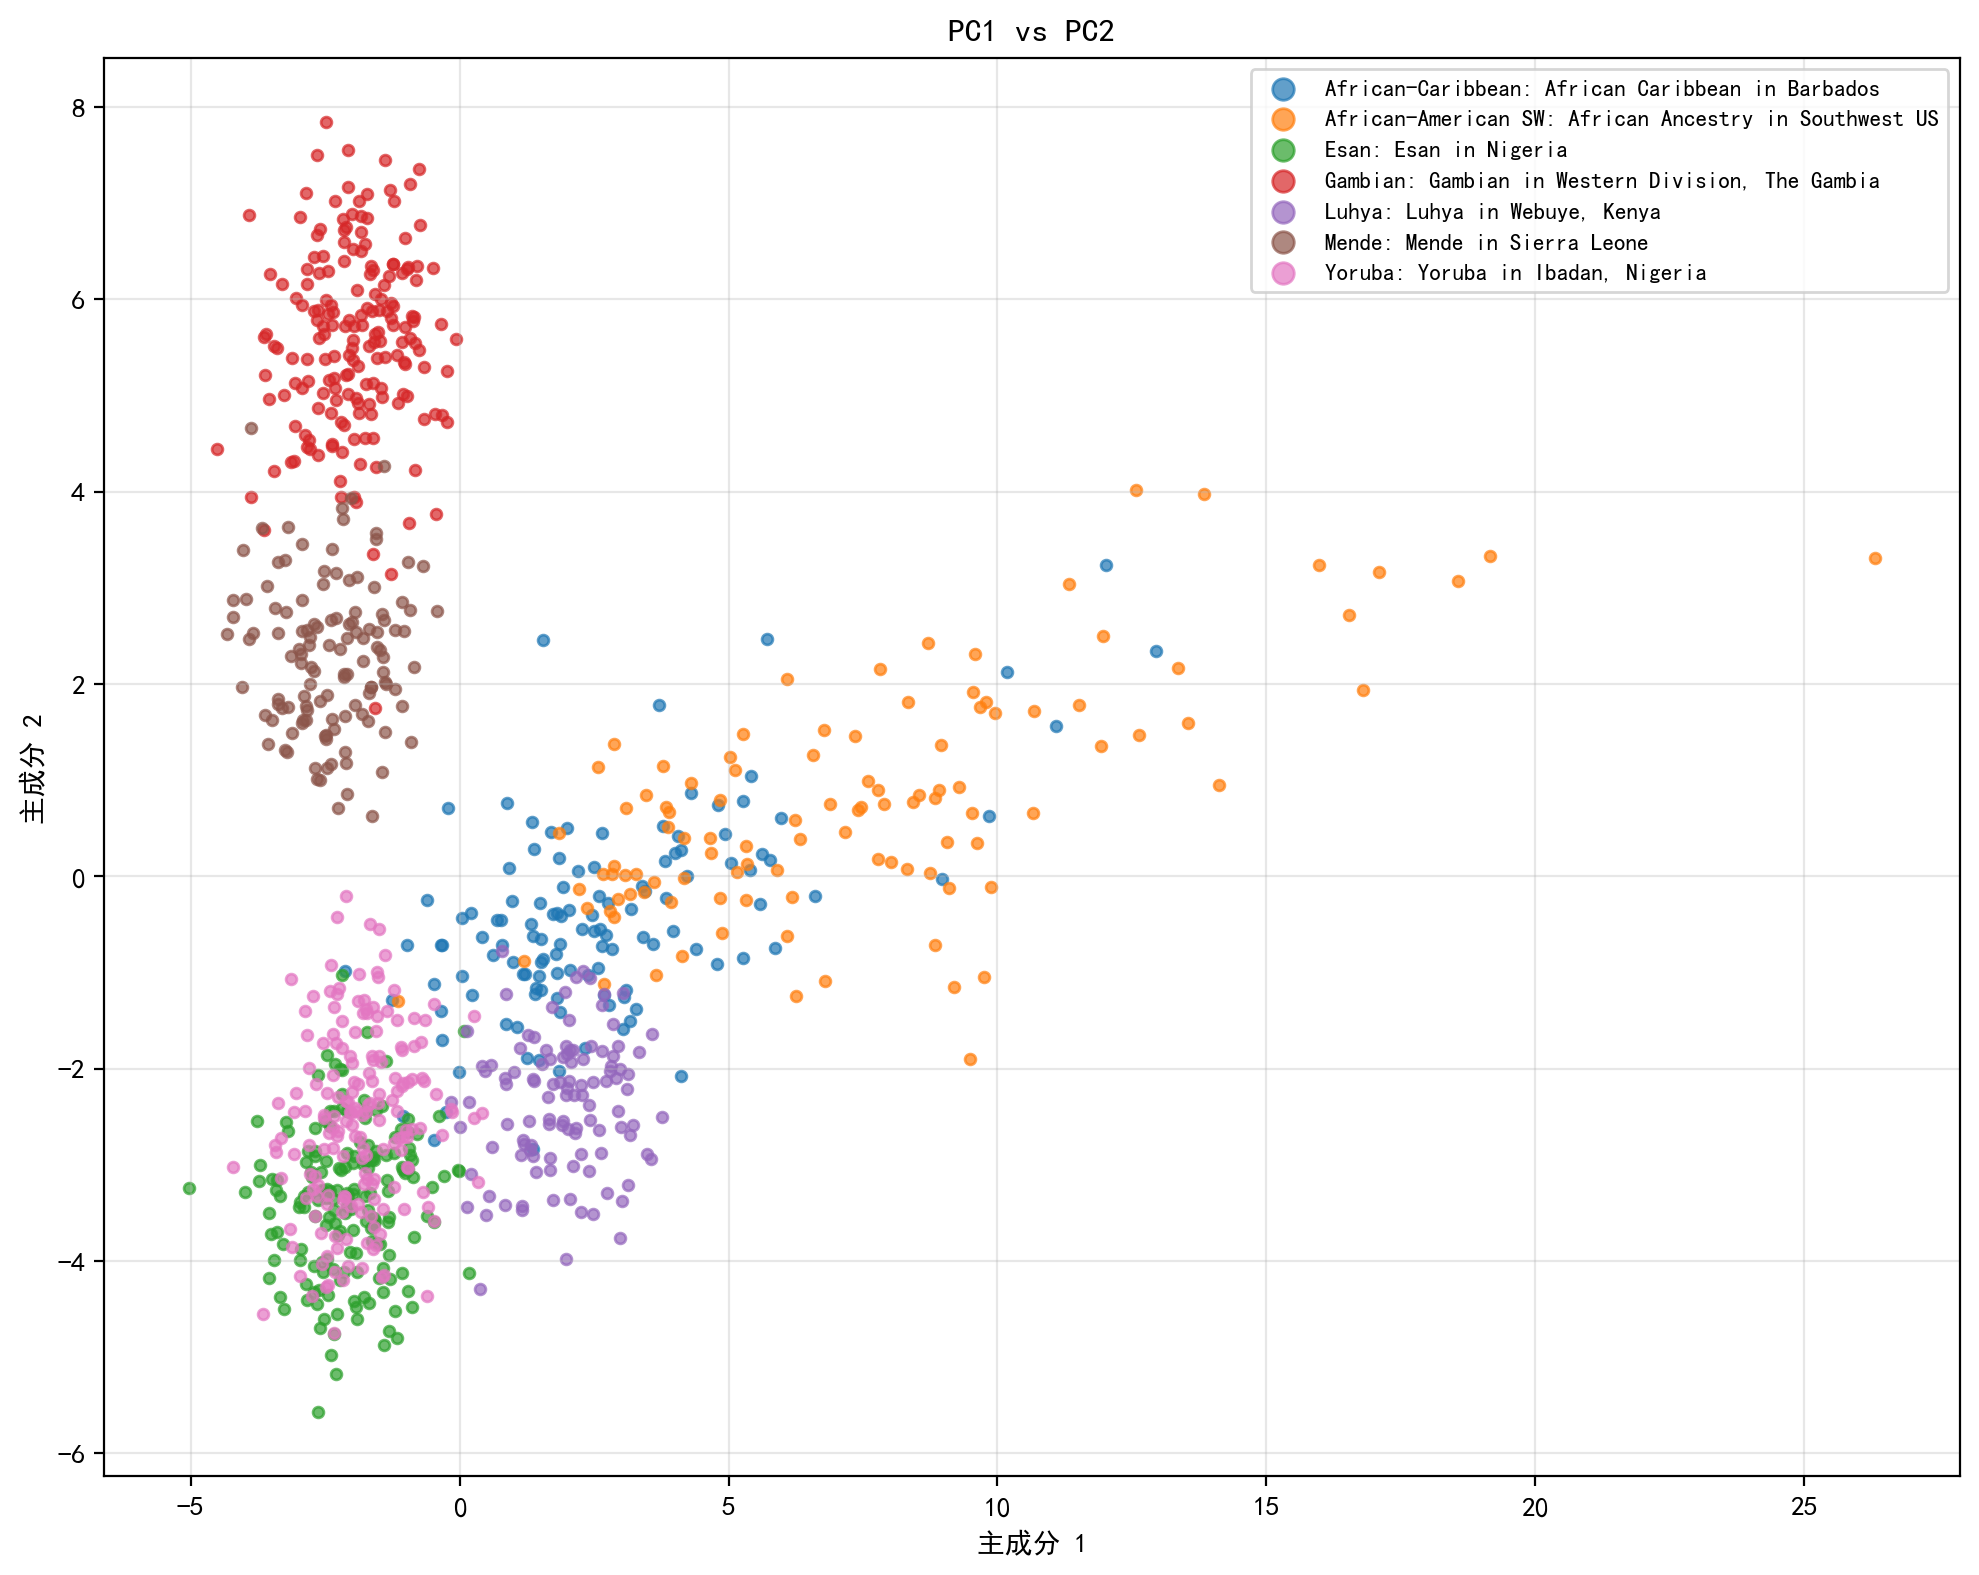
\includegraphics[width=0.8\textwidth]{code/pc1_vs_pc2.png}
    \caption{PC1 vs PC2散点图}
    \label{fig:pc1_pc2}
\end{figure}

\subsection{(c) 前两个主成分特征解释}
从PC1 vs PC2图可以观察到以下重要特征：

\textbf{人群聚类模式}：不同非洲人群在遗传结构上表现出明显的聚类趋势，但同时保持连续的变异模式。其中，非裔美国人群（ASW，橙色）在第一主成分上分布最为分散，显示出与其他非洲人群的显著差异。

\textbf{遗传距离关系}：前两个主成分主要捕获了与地理分布和历史迁徙相关的人群分化信息。西非人群（如YRI、ESN、GWD等）在主成分空间中相对集中，而经历过跨大西洋迁徙和基因混合的人群（如ASW、ACB）则表现出更大的遗传变异范围。

\subsection{(d) 第三主成分分析}
PC1 vs PC3散点图（见图\ref{fig:pc1_pc3}）展示了第一和第三主成分的关系。

\begin{figure}[H]
    \centering
    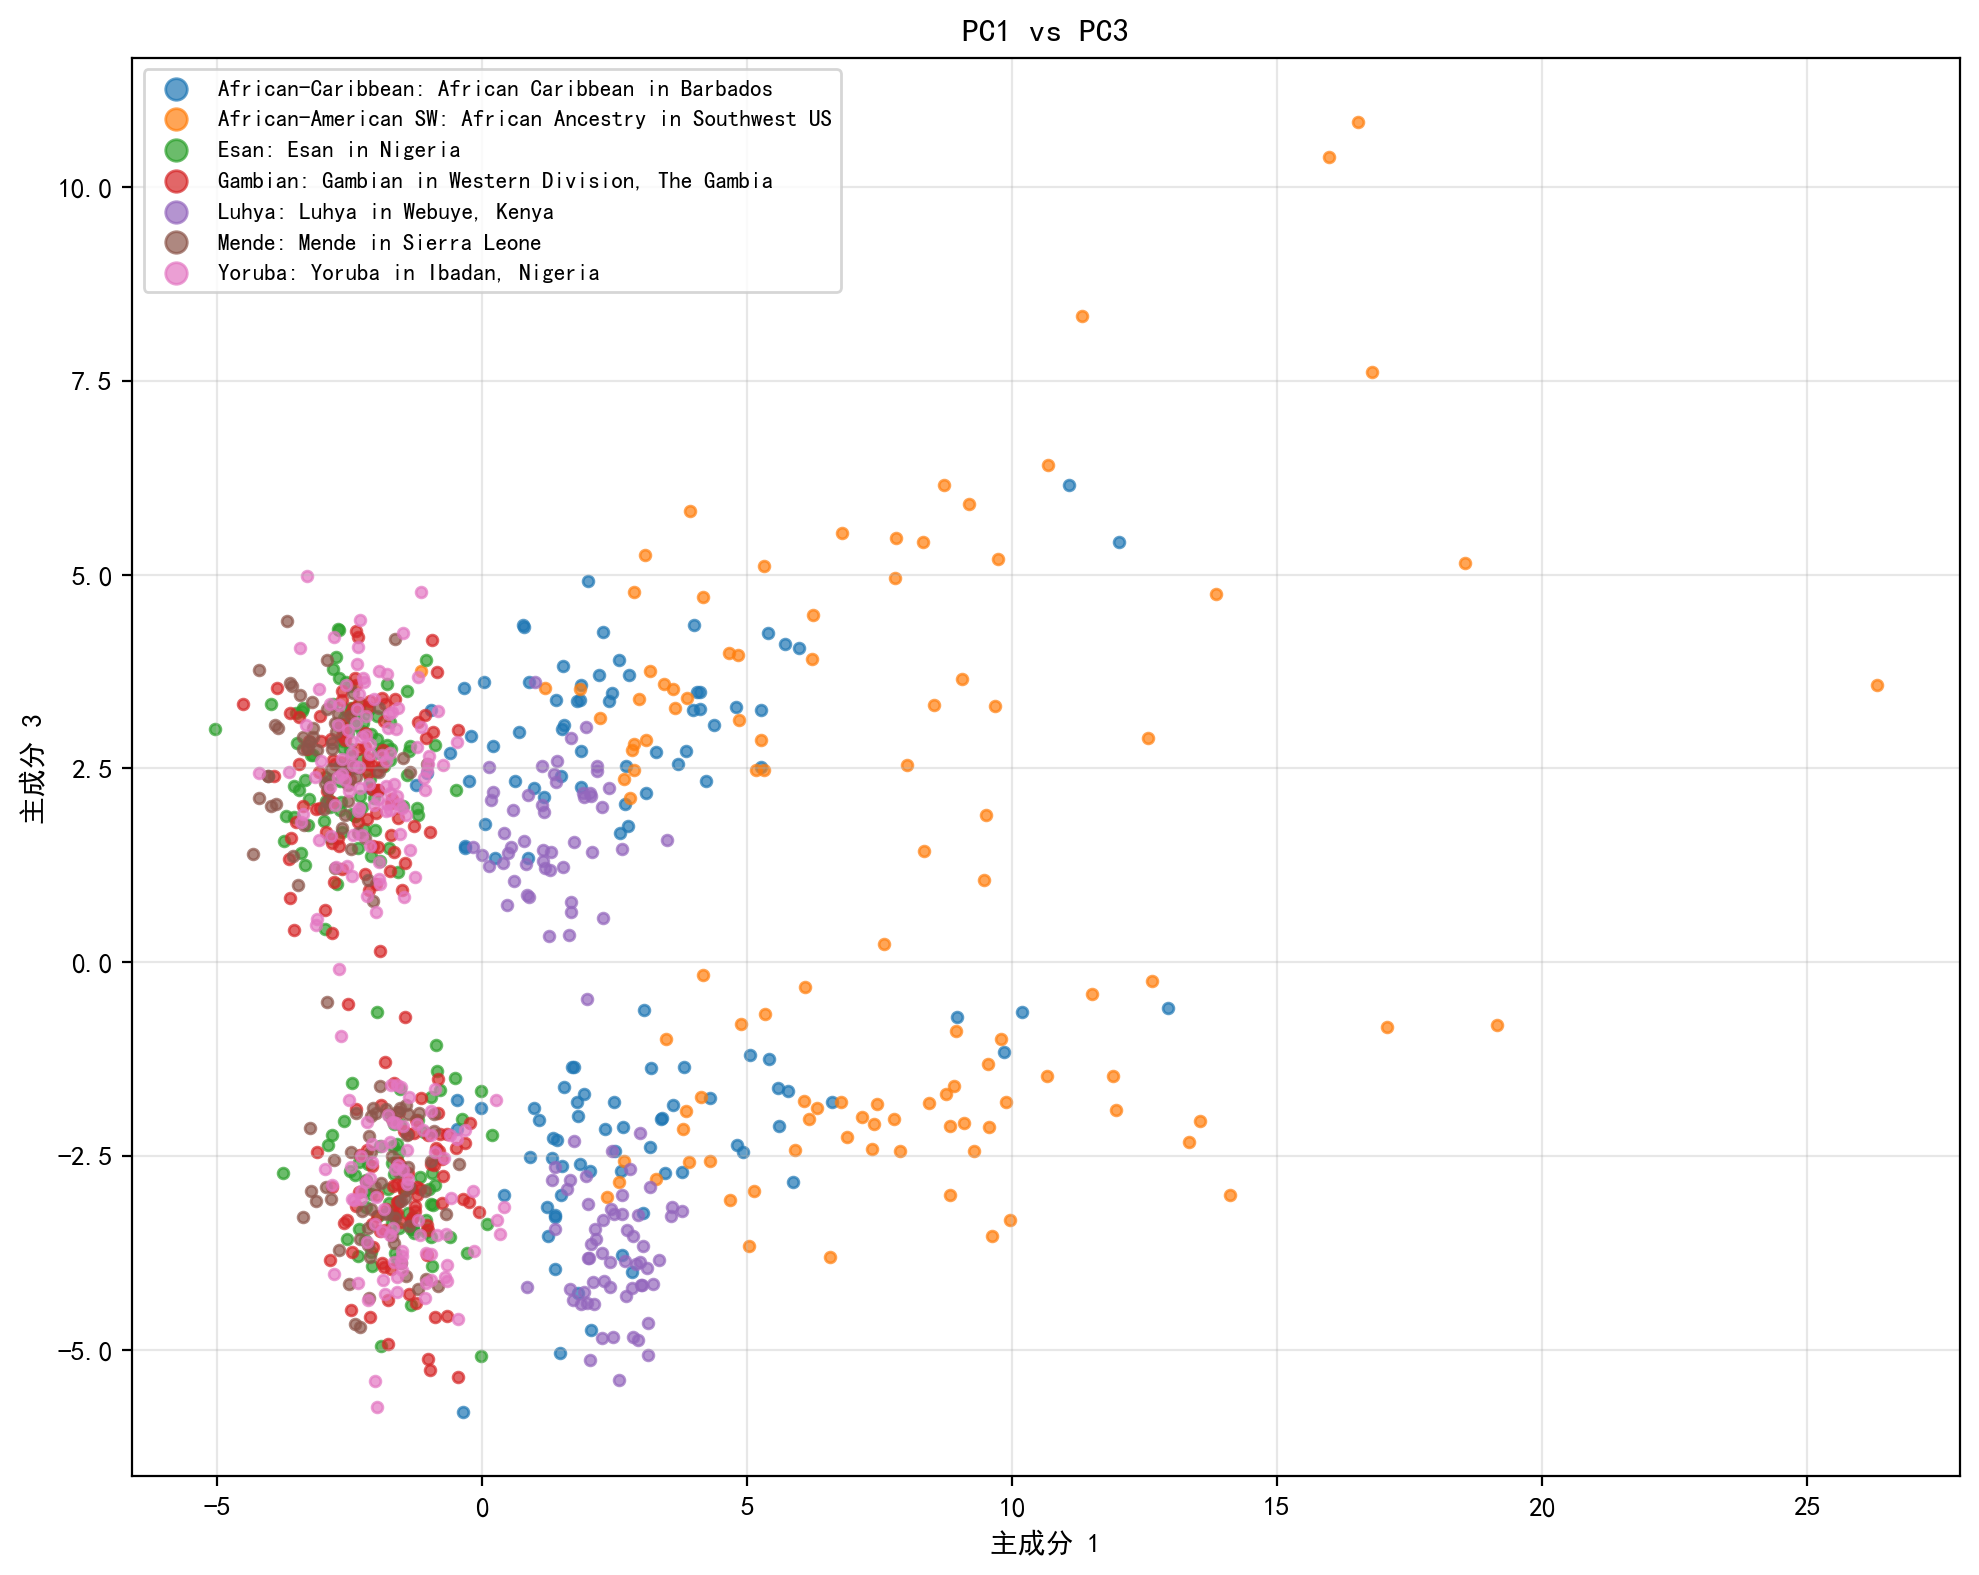
\includegraphics[width=0.8\textwidth]{code/pc1_vs_pc3.png}
    \caption{PC1 vs PC3散点图}
    \label{fig:pc1_pc3}
\end{figure}

\textbf{新的分层模式}：相比PC1 vs PC2图，第三主成分揭示了不同的人群分层模式。部分个体在PC3上表现出极端值，这可能反映了特定的遗传背景或祖先成分的差异。

\textbf{人群细分}：第三主成分进一步细分了在前两个主成分中相对聚集的人群，特别是对非裔美国人群（ASW）的内部结构提供了更细致的解析。

\subsection{(e) 第三主成分含义}
第三主成分可能反映了以下几个方面：
\begin{enumerate}
    \item \textbf{性染色体相关变异}：X/Y染色体上的差异可能导致性别特异性的遗传模式
    \item \textbf{特定基因组区域的选择信号}：某些区域受到自然选择压力，在不同人群中表现出差异
    \item \textbf{人群特有的遗传背景差异}：反映各人群独特的进化历史和遗传漂变
\end{enumerate}

\textbf{注}：由于缺乏SNP的物理位置信息，染色体区域的精确对应需要进一步验证。

\subsection{(f) 第三主成分系数分析}
图\ref{fig:pc3_coeffs}显示了第三主成分系数绝对值随SNP位点索引的变化。

\begin{figure}[H]
    \centering
    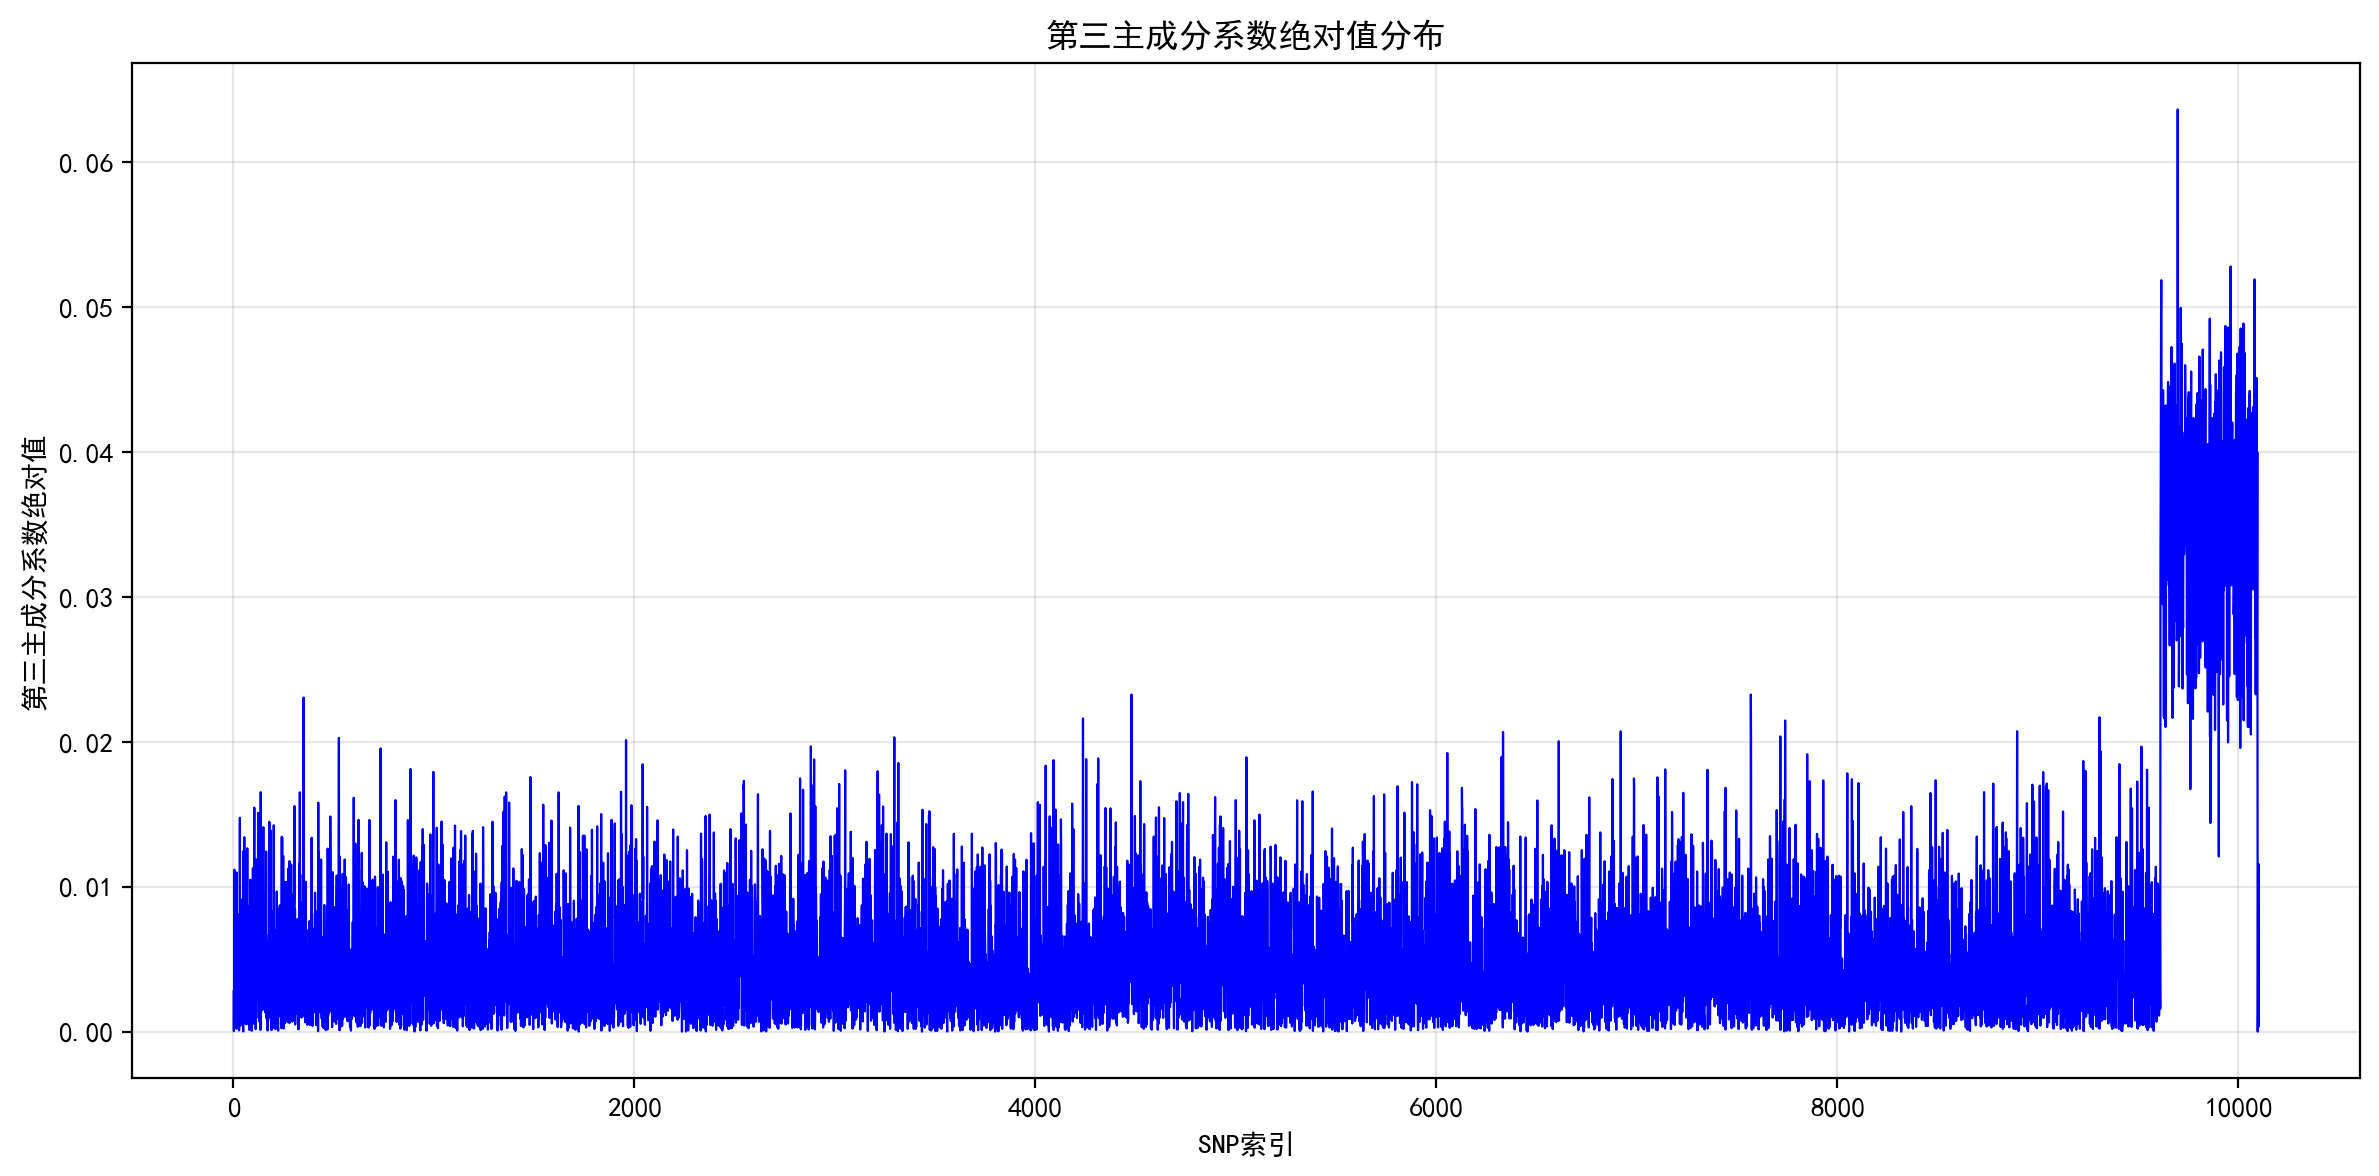
\includegraphics[width=0.8\textwidth]{code/abs_pc3_vs_snpindex.png}
    \caption{第三主成分系数绝对值分布}
    \label{fig:pc3_coeffs}
\end{figure}

\textbf{区域性峰值模式}：从图中可以明显观察到系数值在基因组末端（约9000-10000位点）出现显著的峰值聚集，这一模式具有重要的生物学意义：

\begin{itemize}
    \item \textbf{染色体边界效应}：峰值区域可能对应特定染色体的端粒区或着丝粒附近区域，这些区域通常具有特殊的遗传重组模式
    \item \textbf{连锁不平衡}：连续的高值区域表明存在强连锁不平衡，暗示这些SNP位点在进化过程中作为一个单元传递
    \item \textbf{选择信号}：局部峰值可能反映了特定基因区域受到的选择压力，导致该区域在不同人群间表现出差异化的等位基因频率
\end{itemize}

\subsection{(g) 方差解释分析}
\begin{itemize}
    \item 第一主成分解释的方差百分比：\textbf{0.57\%}
    \item 前3个主成分解释的总方差百分比：\textbf{1.41\%}
\end{itemize}

\textbf{结果讨论}：

虽然解释方差比例较低，但这符合高维基因组数据的特性，具体原因如下：

\begin{itemize}
    \item \textbf{高维数据特性}：在10,101个SNP位点构成的高维空间中，即使很小的方差比例也能捕获重要的生物学信号。这是高维数据分析的典型特征。
    
    \item \textbf{群体遗传学原理}：根据人类遗传学研究，约85-90\%的遗传变异存在于个体内部，仅10-15\%的变异用于区分不同人群。我们观察到的低方差解释比例与这一原理高度一致。
    
    \item \textbf{非洲人群特殊性}：本研究的所有样本均来自非洲及非洲裔人群。作为现代人类的起源地，非洲人群内部遗传多样性高但人群间分化相对较小，这进一步降低了主成分能够解释的方差比例。
    
    \item \textbf{有效性验证}：尽管方差解释比例较小，但从散点图可以清楚看到不同人群的聚类模式，说明PCA成功捕获了关键的人群结构信息。这证明了该方法在基因组数据分析中的有效性。
\end{itemize}

\textbf{结论}：低方差解释比例不仅合理，而且符合预期，反映了基因组数据分析的固有特性和人类遗传变异的基本模式。

\section{总结反思}

\subsection{主要发现}
\begin{enumerate}
    \item \textbf{人群结构清晰}：PCA成功揭示了非洲及非洲裔人群的遗传结构，不同人群在主成分空间中表现出明显的聚类模式
    \item \textbf{历史迁徙印记}：非裔美国人群（ASW）的分散分布反映了跨大西洋奴隶贸易和随后的基因混合历史
    \item \textbf{基因组区域差异}：第三主成分系数分析揭示了基因组中不同区域对人群分化的不均等贡献
    \item \textbf{方法有效性}：即使在低方差解释比例下，PCA仍能有效提取人群遗传结构信息
\end{enumerate}

\subsection{生物学意义}
本研究的结果与现有的人类遗传学知识高度一致：
\begin{itemize}
    \item 证实了非洲大陆作为现代人类起源地的高遗传多样性
    \item 揭示了历史人口迁徙和混合事件在基因组中留下的印记
    \item 展示了不同染色体区域在人群分化过程中的不同作用
\end{itemize}

\subsection{技术反思}
\begin{itemize}
    \item \textbf{数据预处理}：二值化编码策略有效地将离散核苷酸数据转换为适合PCA分析的连续数值
    \item \textbf{降维效果}：PCA成功将10,101维数据降至低维空间，同时保留了关键的生物学信息
    \item \textbf{可视化价值}：主成分散点图为理解复杂的高维遗传数据提供了直观的可视化手段
\end{itemize}

\end{document}